\documentclass[master.tex]{subfiles}

\begin{document}

\section*{C. Preliminary Studies}

\subsection*{Retrospective memory linking window is longer than prospective
  linking window for a negative memory}

\begin{wrapfigure}{r}{0.6\textwidth}
  \centering 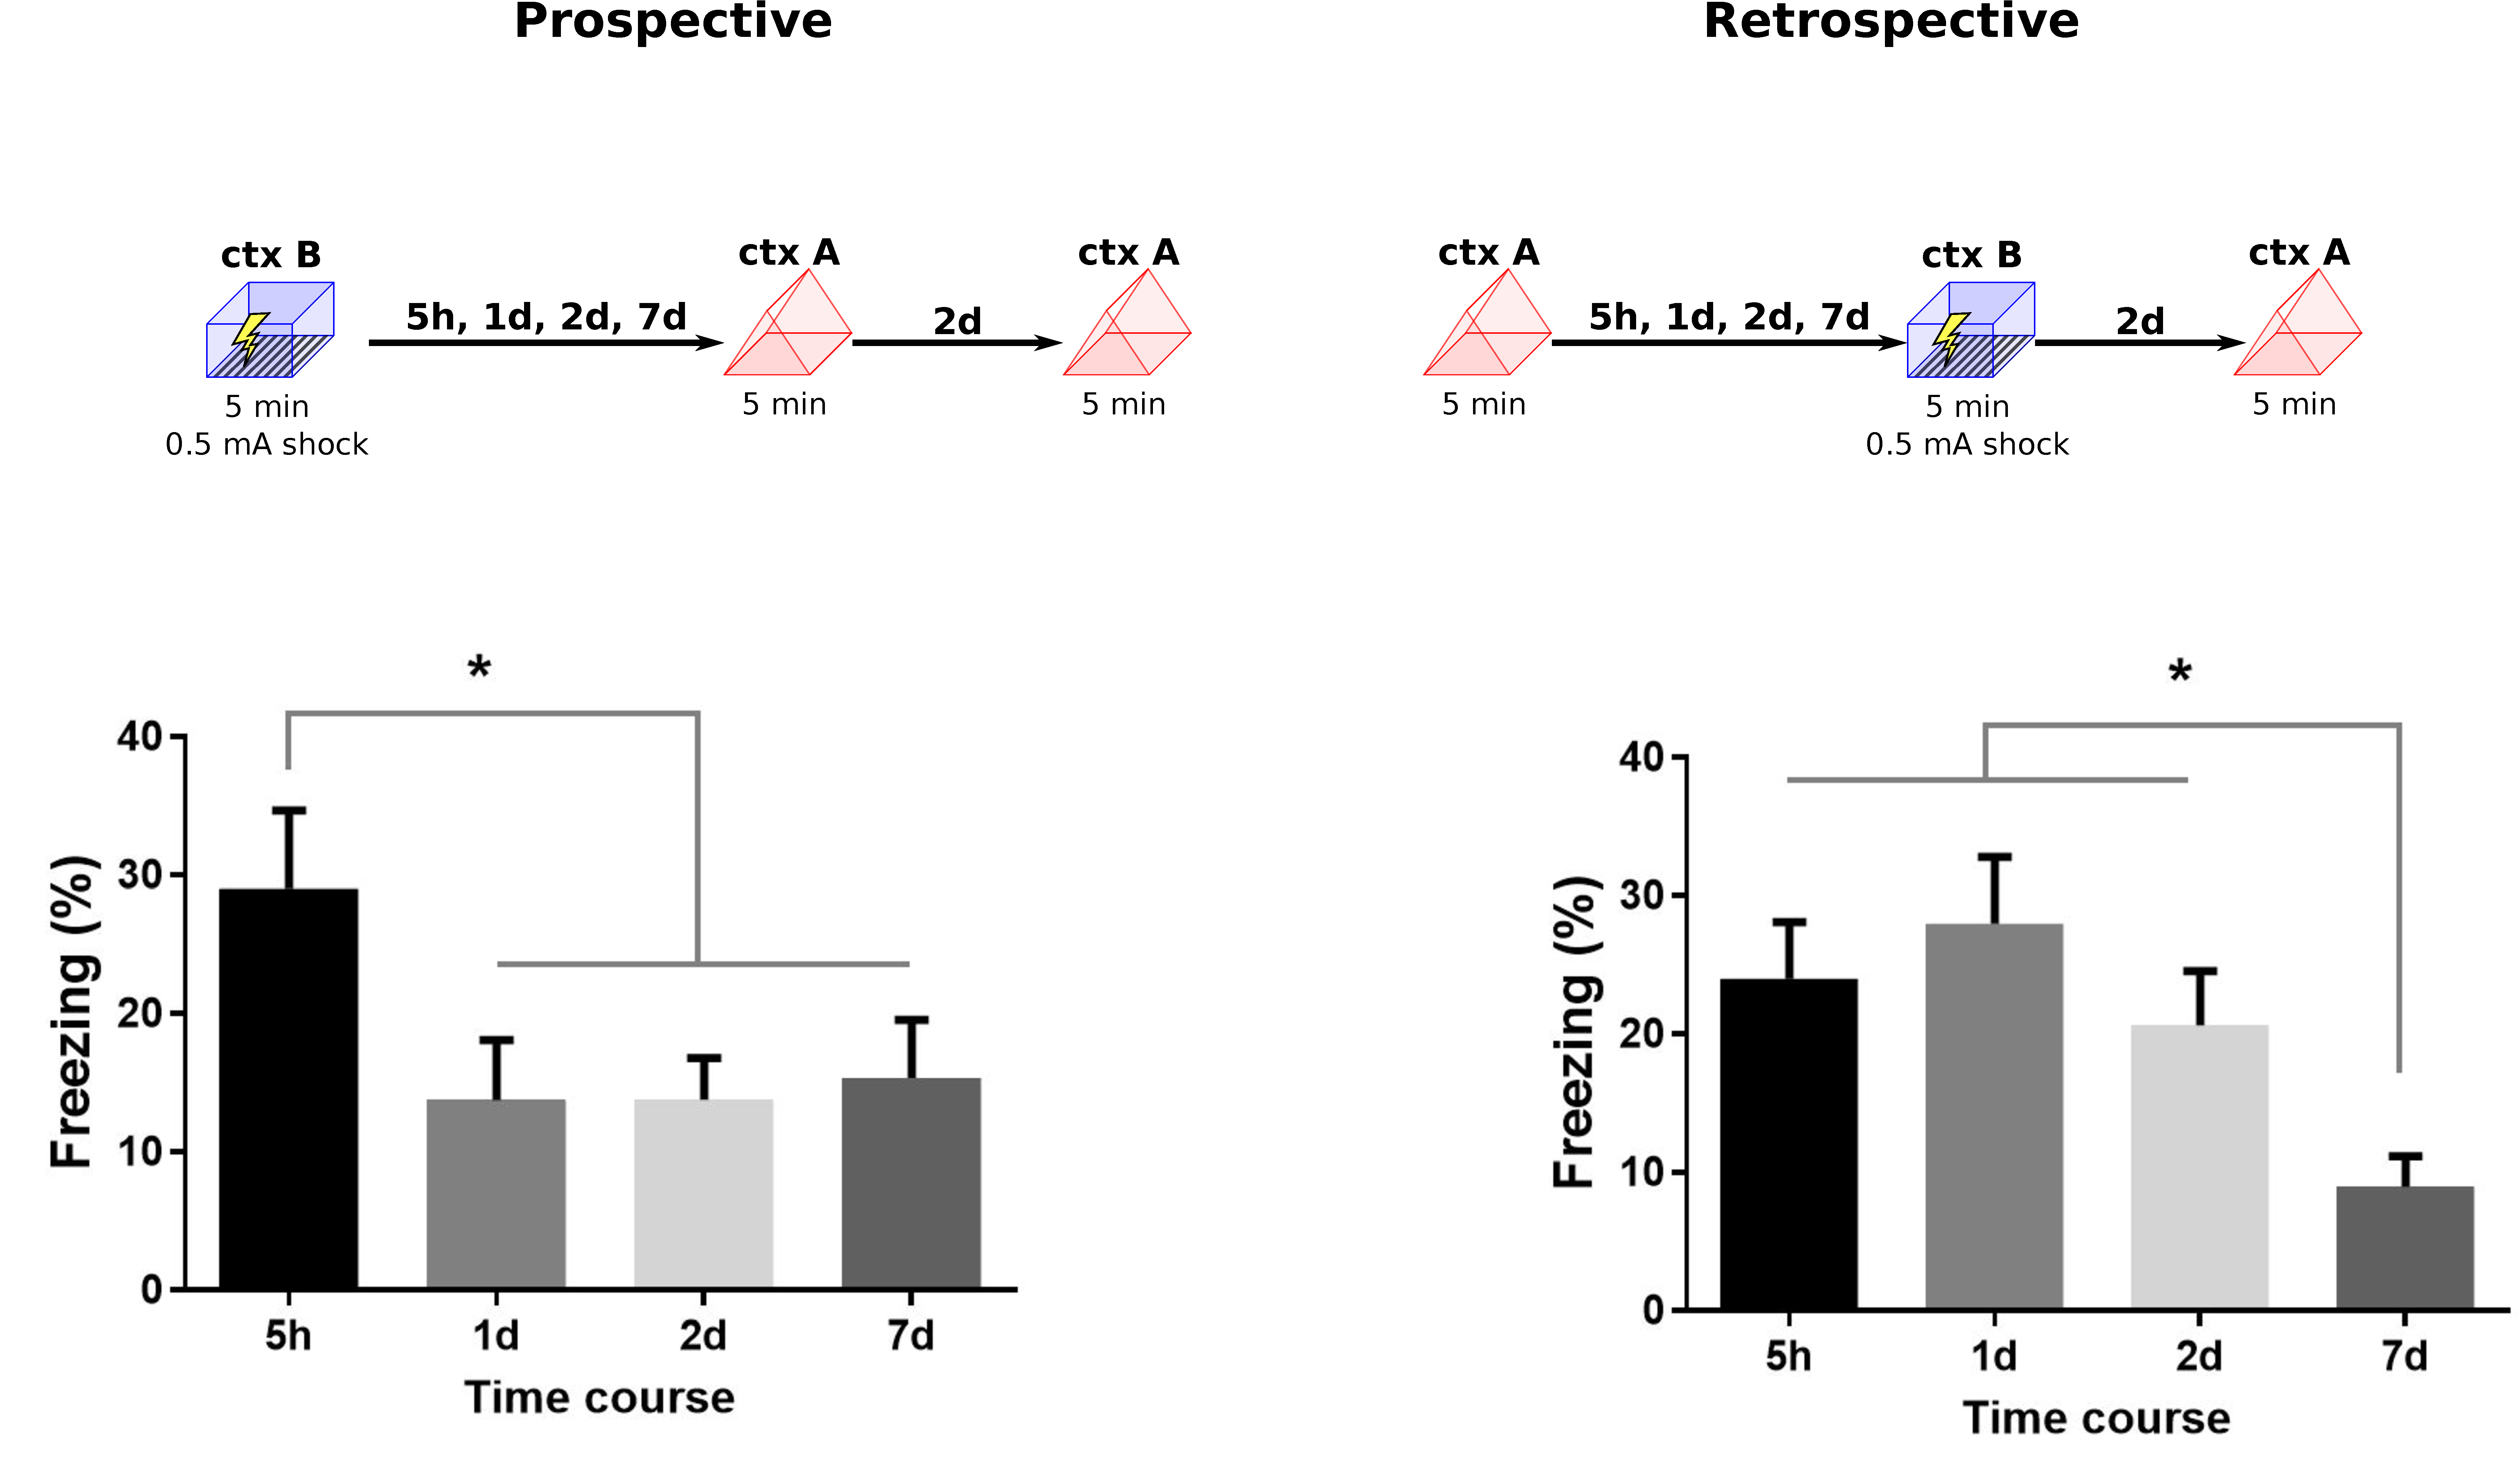
\includegraphics[scale = .095]{Figures/pro_retro_prelim.pdf}
  \caption{\footnotesize Retrospective memory linking window is longer than
    prospective linking window for a negative memory.}
  \label{fig:prelim_pro_retro}
\end{wrapfigure}

% \begin{figure}[!h]
%   \centering 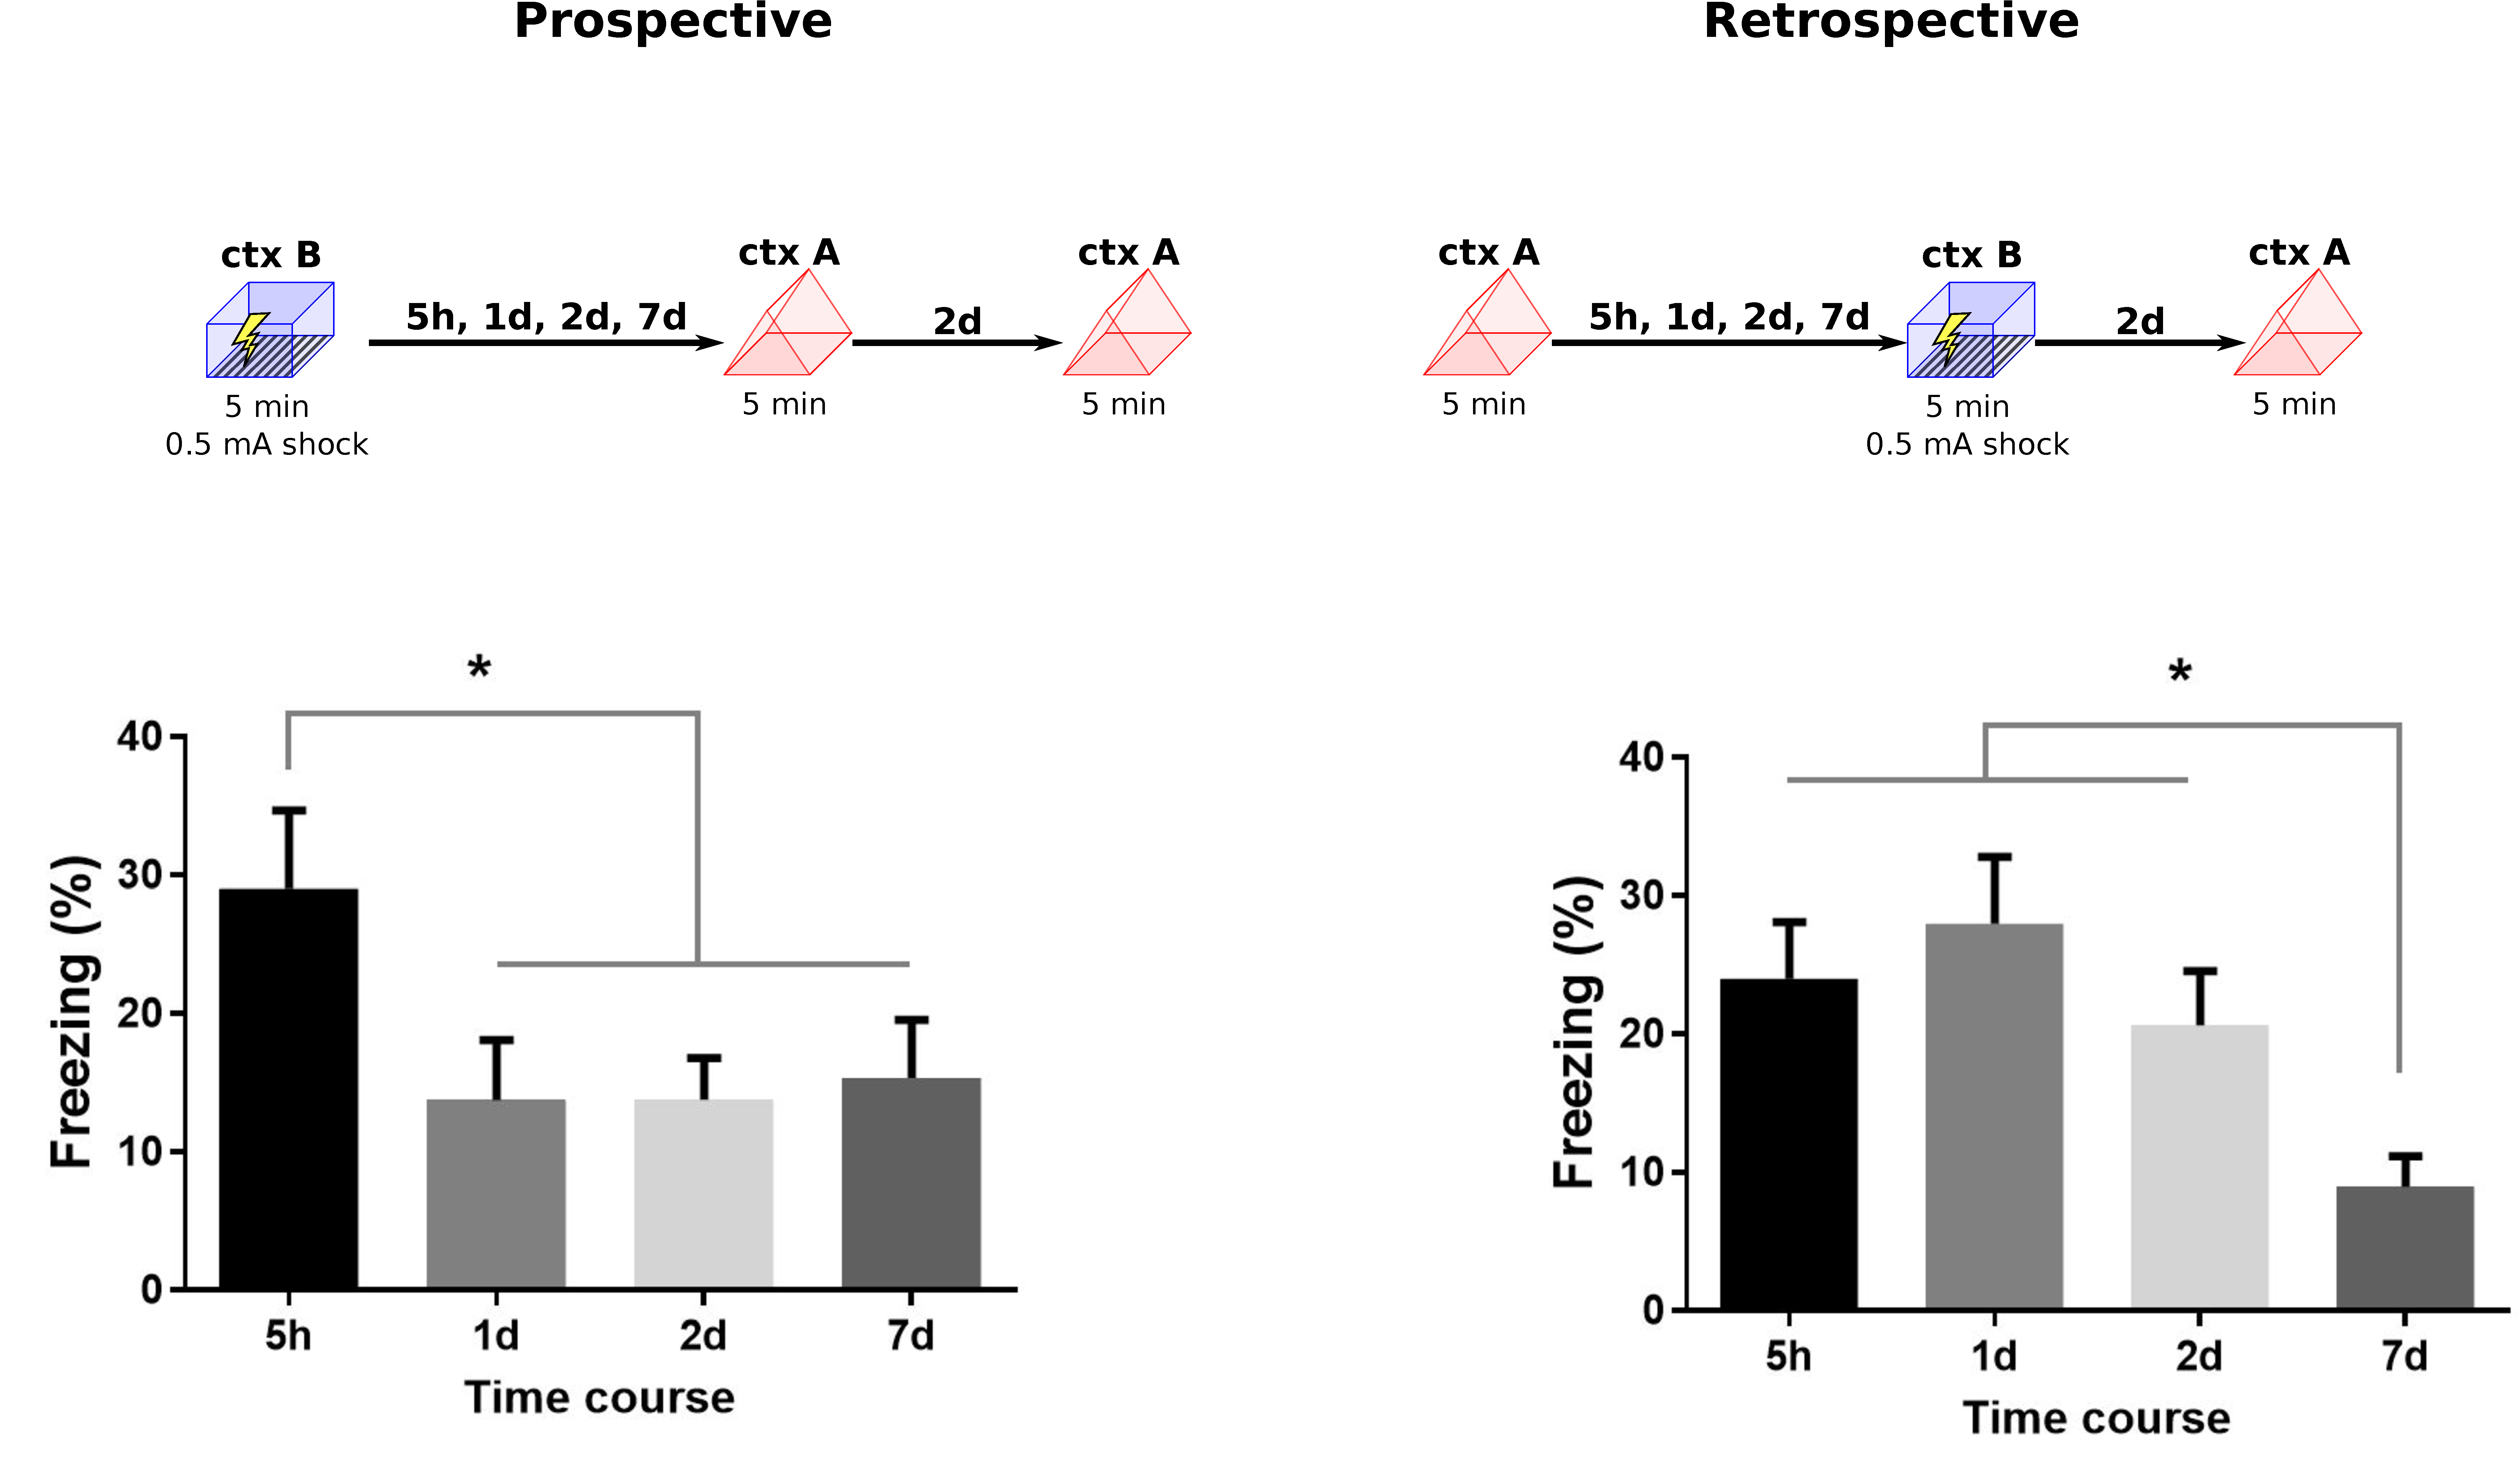
\includegraphics[scale = .15]{Figures/pro_retro_prelim.pdf}
%   \caption{\footnotesize Retrospective memory linking window is longer than
%   prospective linking window for a negative memory.}
%   \label{fig:prelim_pro_retro}
% \end{figure}

In the preliminary study shown in \autoref{fig:prelim_pro_retro}, animals were
put into two distinct contexts and separated into two major groups for which the
temporal order of the two contexts during encoding is opposite. In the
``prospective'' group, animals received a delayed shock in context B first, and
then explore context A, whereas in the ``retrospective'' group, animals explored
context A first, and then get a delayed shock in context B. Both groups were
tested in context A again 2 days after they are exposed to both context A and B.
Within each major group, the animals were further divided into subgroups in
which exposure to A and B were separated by varying intervals of time. Thus,
elevated freezing level in the context A, where no shock ever occurred for both
groups, indicates a transfer of fear and a linking of the two contexts.
Furthermore, comparison of freezing levels in context A between subgroups with
various time intervals can reveal the difference of temporal windows of memory
linking across ``prospective'' and ``retrospective'' groups. For all groups, the
exploration and testing session lasted for 5 minutes, a foot shock of 0.5 mA was
delivered at the beginning of the second minute. The various time intervals are
5 hours, 1 day, 2 days and 7 days for both groups.

In the ``prospective'' linking group, we observed significant higher freezing level
in context A with 5 hours interval relative to those with 7 day interval, but
not with either 1 day or 2 days interval. This suggest that the fear memories
were able to transfer forward to a neutral context 5 hours in the future. On the
other hand, in the ``retrospective'' linking group, we observed higher freezing
level with 5 hours, 1 day and 2 days interval compared to those with 7 days
interval. This suggests that fear memory was able to transfer backward up to 2
days. Taken together, these results suggest an extended temporal window of
retrospective memory linking compared to prospective memory linking.

\subsection*{The difference in overlap of ensembles across groups emerge after
  encoding}

\begin{wrapfigure}{l}{0.6\textwidth}
  \centering 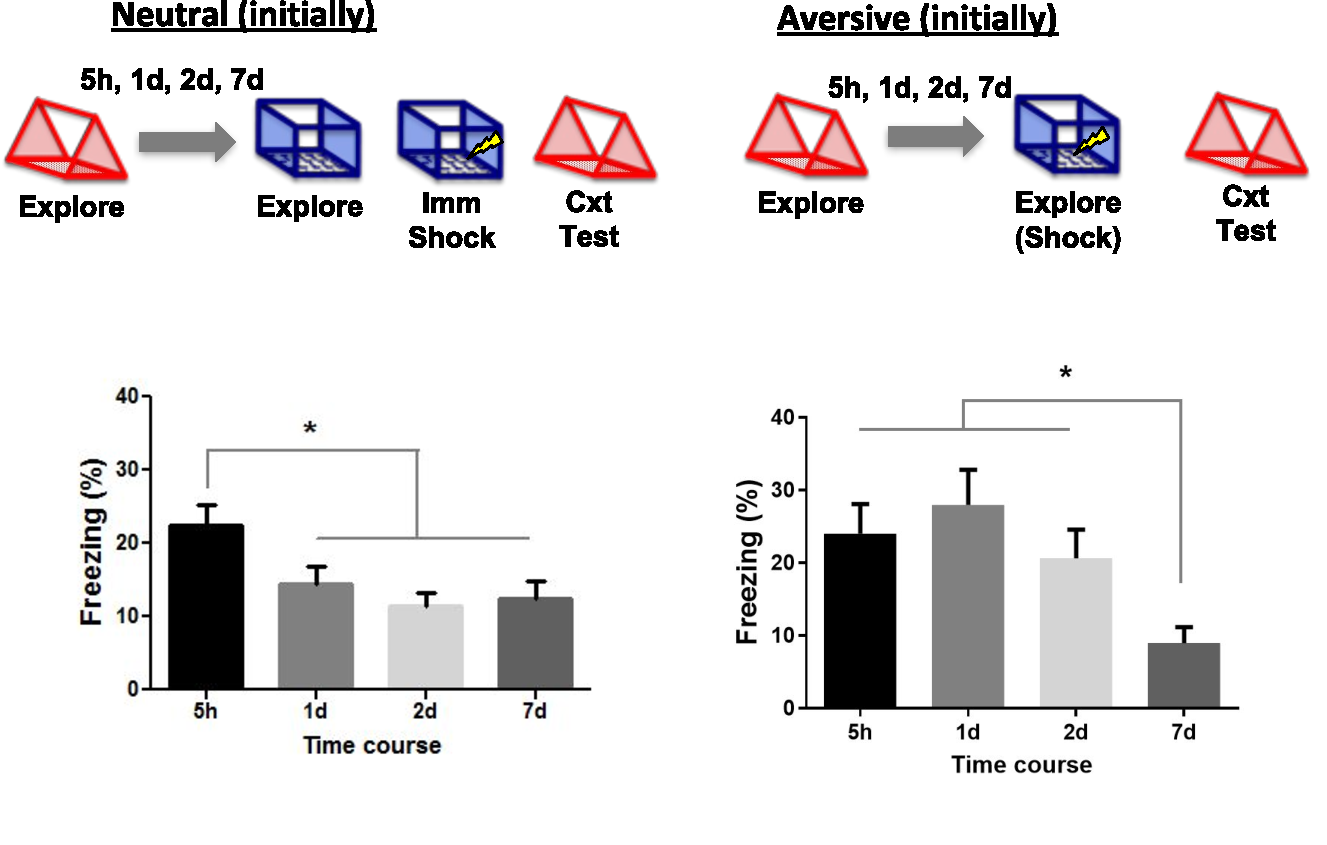
\includegraphics[scale = .095]{Figures/val_retro_prelim.pdf}
  \caption{\footnotesize Negative valence increased temporal window of memory
    linking.}
  \label{fig:prelim_val}
\end{wrapfigure}

% \begin{figure}[!h]
%   \centering 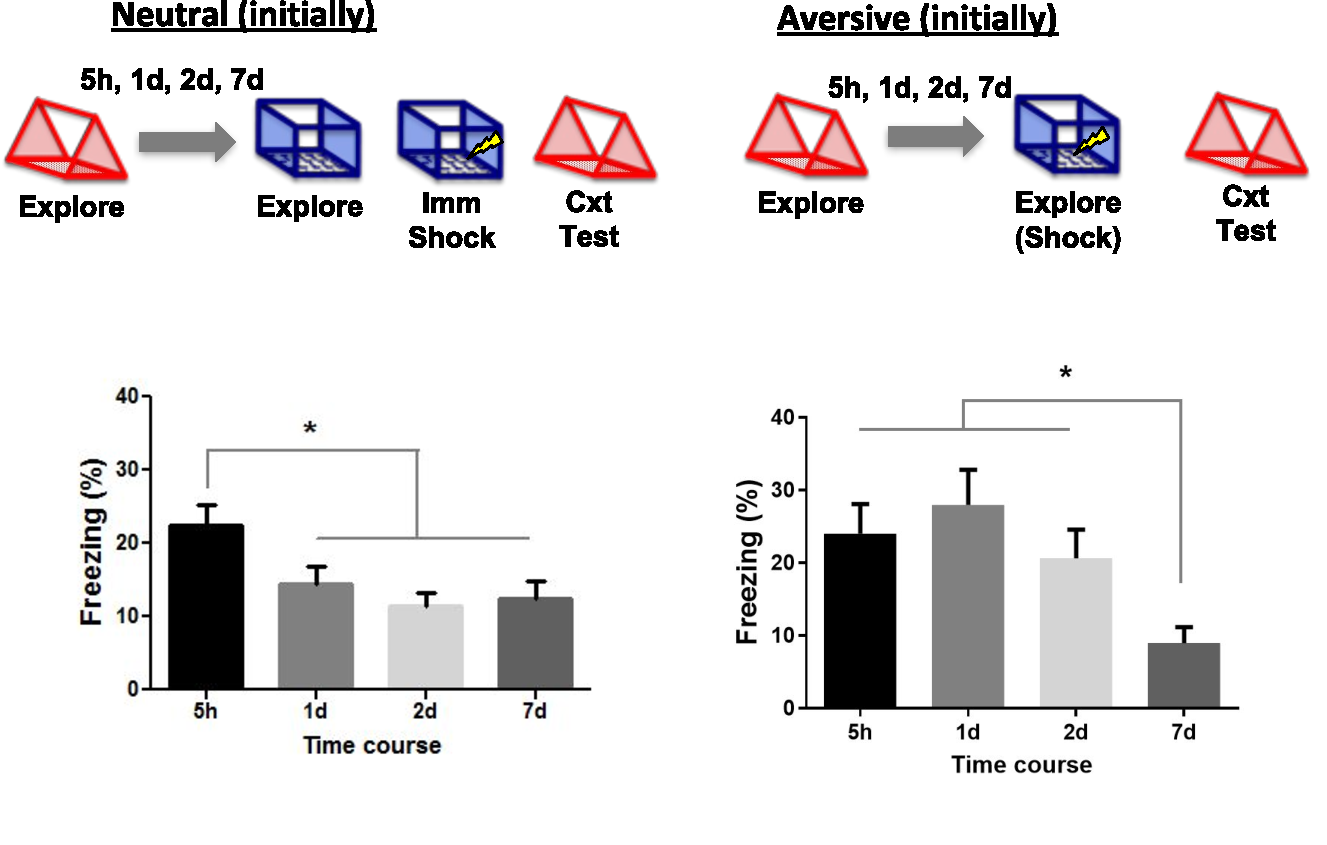
\includegraphics[scale = .15]{Figures/val_retro_prelim.pdf}
%   \caption{\footnotesize Negative valence increased temporal window of memory
%   linking.}
%   \label{fig:prelim_val}
% \end{figure}


In the preliminary study shown in \autoref{fig:prelim_val}, the effect of
negative valence on the temporal window of retrospective memory linking was
studied. Briefly, animals were put into context A and B in that order and were
divided into two major groups --- ``neutral'' and ``aversive''. The difference
between the two major groups is that in the ``aversive'' group, the animals
received a delayed shock during the encoding session of context B, thus making
context B an aversive memory from the beginning. In contrast, for the
``neutral'' group, the emotional valence of context B was initially neutral, and
the animals received an immediate shock 2 days after the initial exploration of
context B. Similar to the preliminary experiments described earlier, animals
within each major group were further divided into sub groups according to various
time intervals between initial exposure of context A and B, while all of the
animals were put back to context A for testing and the comparison of freezing
levels in A between sub groups could reveal the difference in temporal windows
of memory linking across ``neutral'' and ``aversive'' groups. We observed that
consistent with published works, animals in the ``neutral'' group can only link
the two memories across 5 hours. However, animals in the ``aversive'' group can
link the two memories across 2 days, suggesting an extension of temporal window
of memory linking due to emotional valence of the initial context memory. Thus,
we chose a temporal interval of 2 days for following calcium imaging studies,
since there was a significant difference in behavior across the two groups with a
2 day time interval.

\begin{wrapfigure}{r}{0.6\textwidth}
  \centering 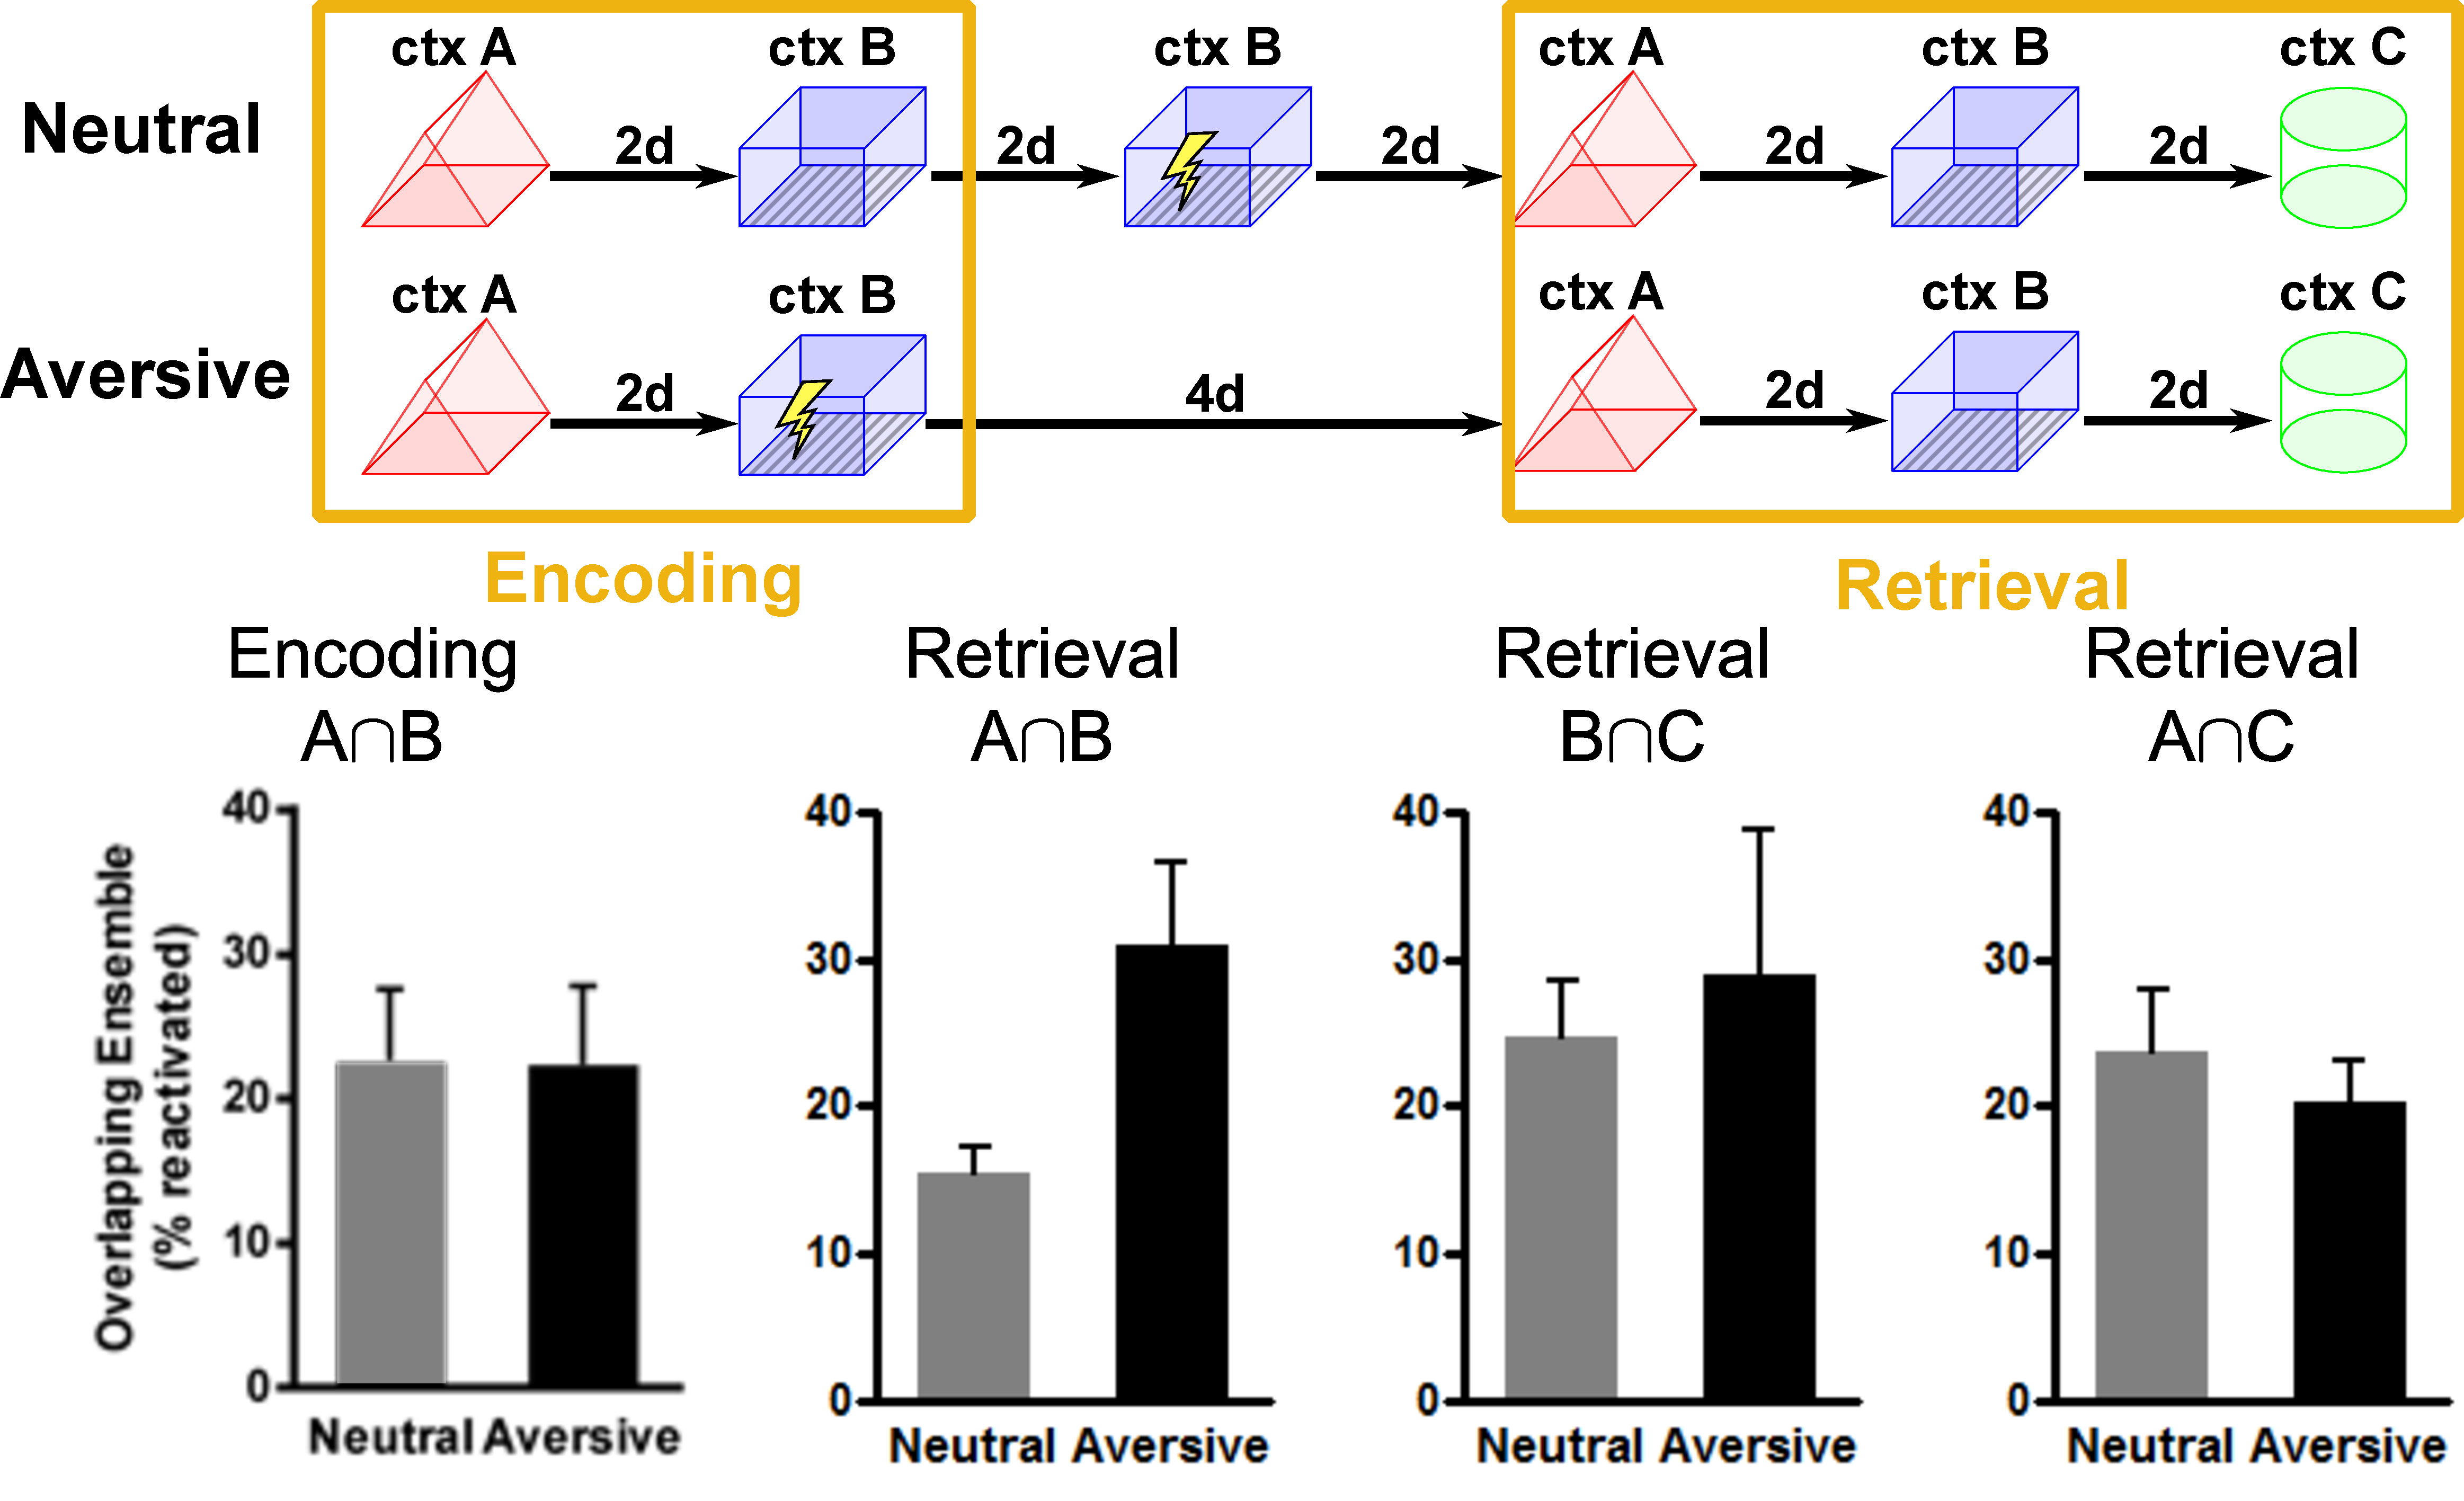
\includegraphics[scale = .09]{Figures/val_retro_prelim_imag.pdf}
  \caption{\footnotesize Increase in ensemble overlap emerges after encoding.}
  \label{fig:prelim_val_imag}
\end{wrapfigure}

% \begin{figure}[!h]
%   \centering 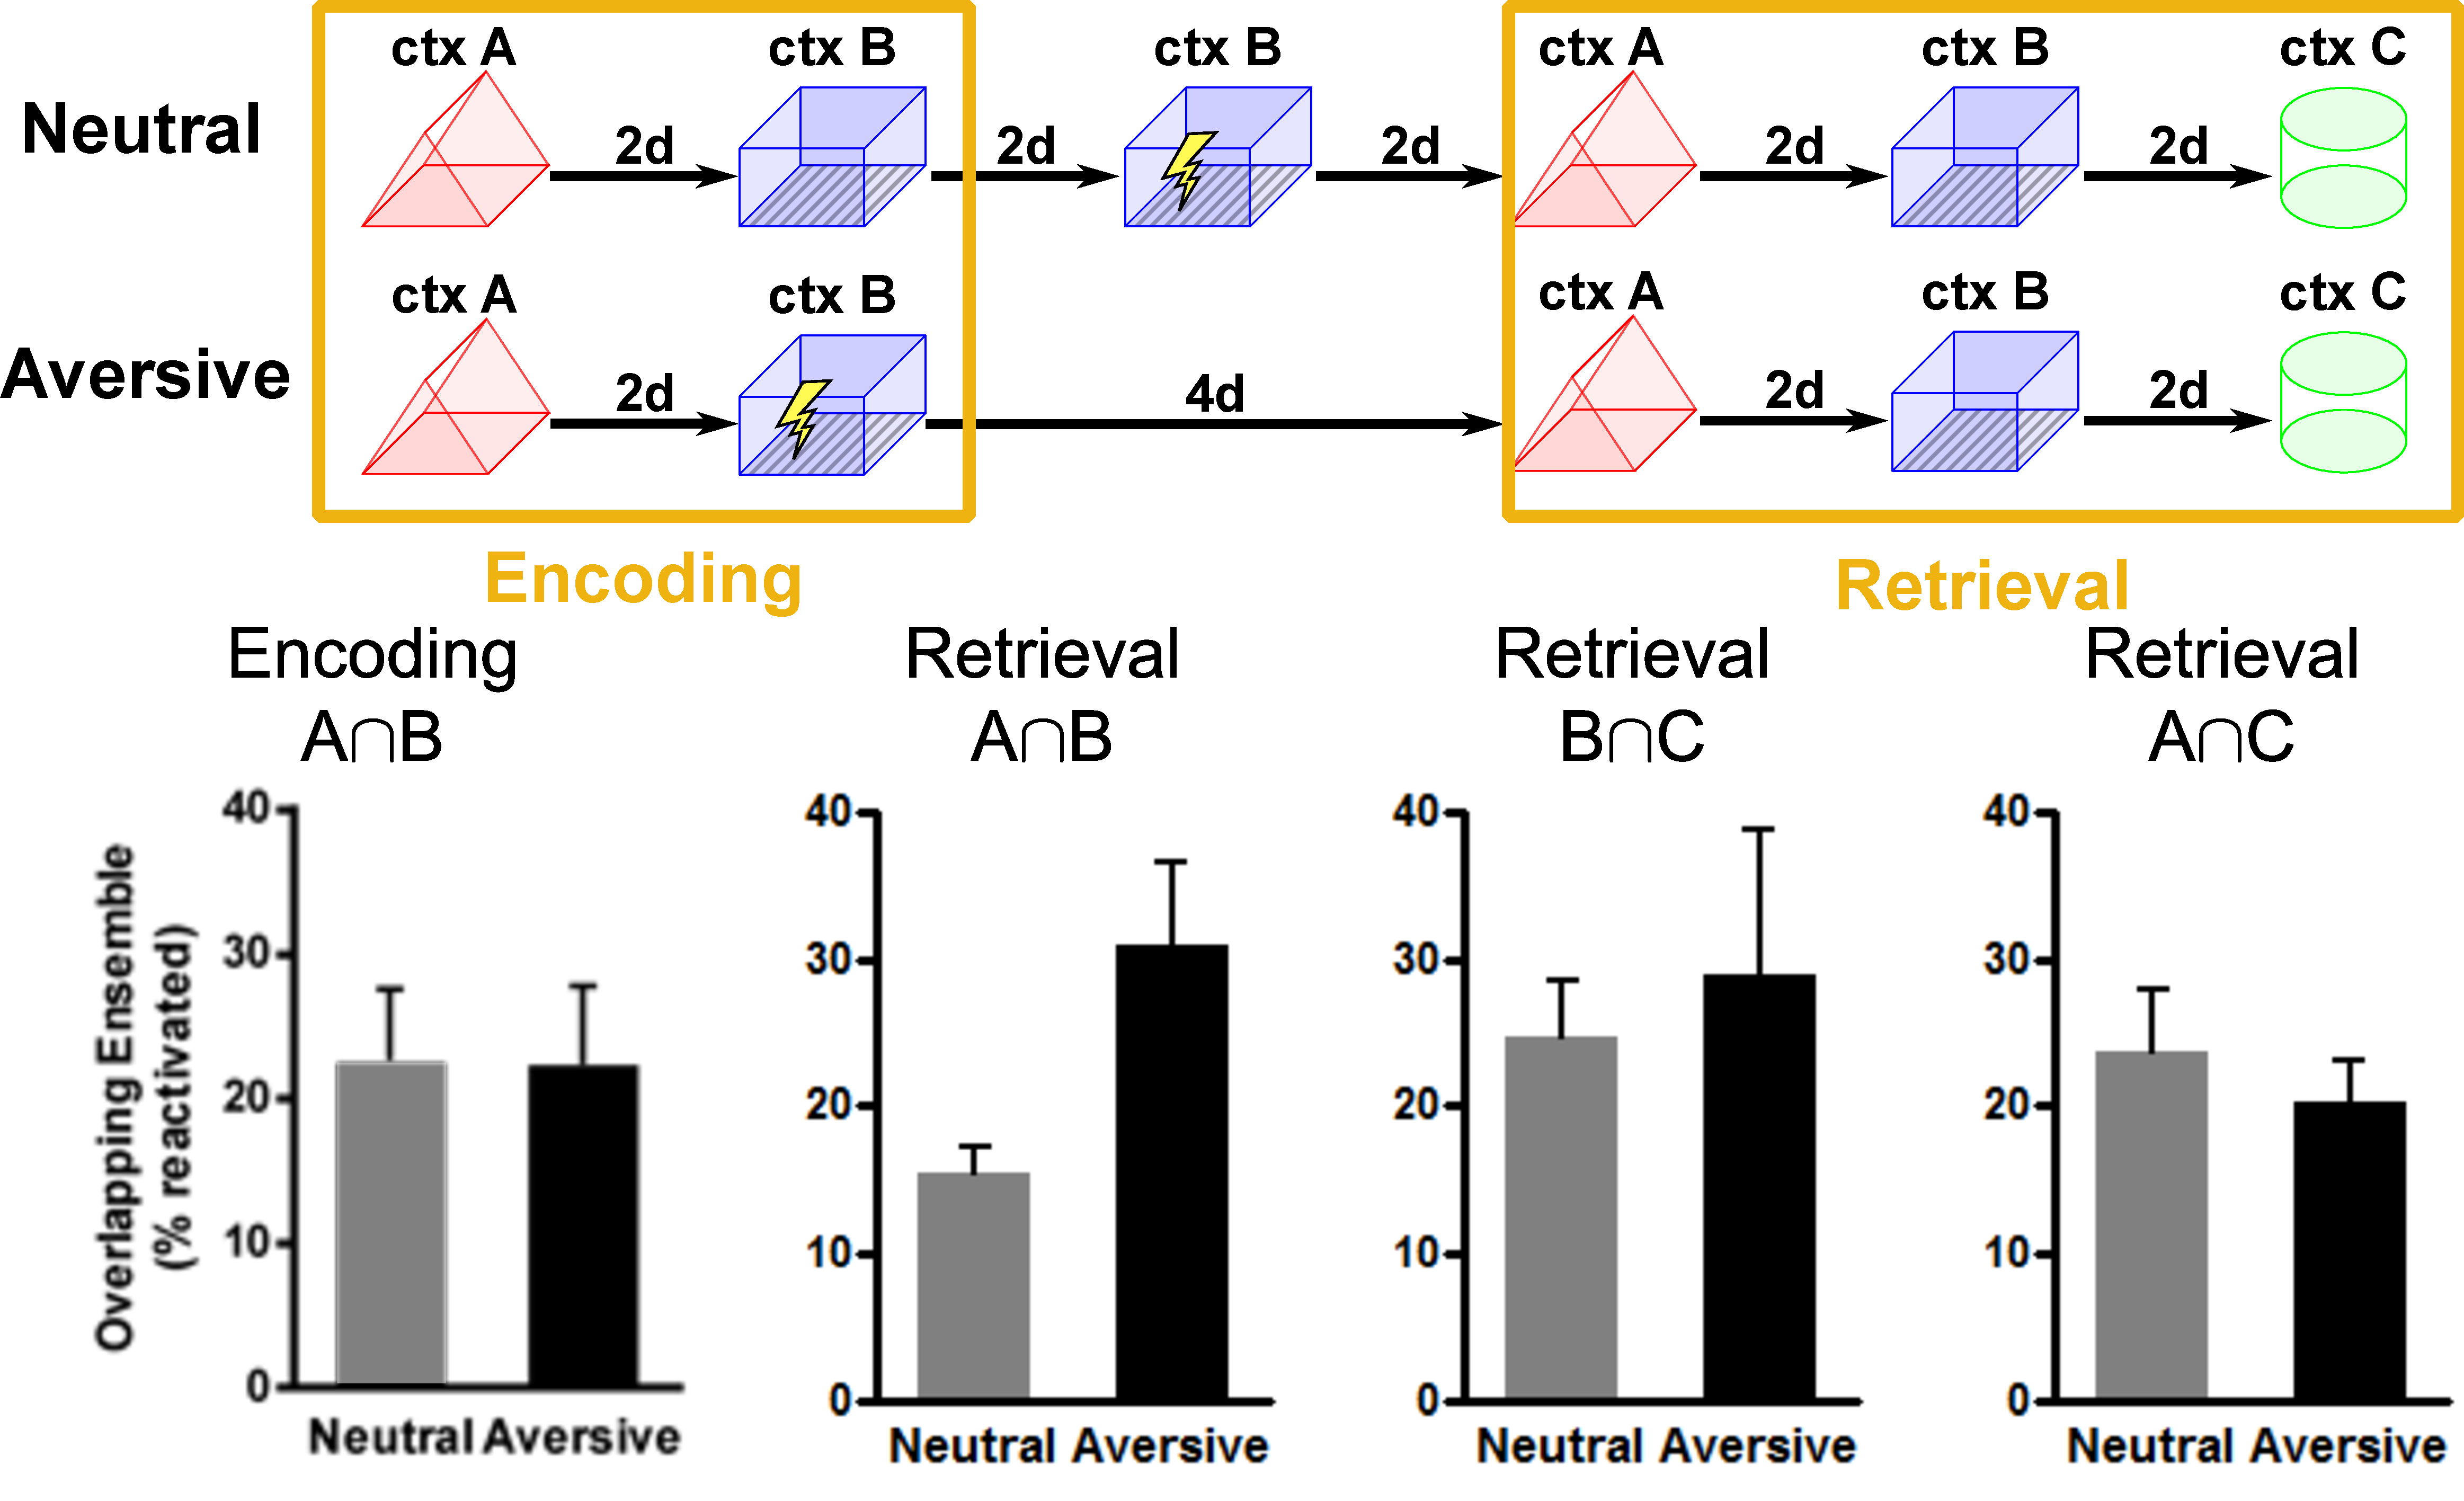
\includegraphics[scale = .15]{Figures/val_retro_prelim_imag.pdf}
%   \caption{\footnotesize Increase in ensemble overlap emerges after encoding.}
%   \label{fig:prelim_val_imag}
% \end{figure}

In the accompanying imaging study shown in \autoref{fig:prelim_val_imag}, the
animals were divided into two groups and undergo the same paradigm as described
above. The difference is that the time interval between context A and B is set
to 2 days for all animals, and that animals are tested in a novel context C in
addition to context A. Calcium imaging with miniature microscope was carried out in all
sessions, so that the neural ensemble of each session can be obtained and comparisons
of ensembles can be carried out within subject. Specifically, we looked at the
overlap between two ensembles, which is the number of neurons that were active
in both sessions as a proportion of the total number of neurons that were active in
either sessions. Consistent with behavioral results, during retrieval, we observed
a significant increase in the overlap between ensembles of context A and B in
the ``aversive'' group, but not in the ``neutral'' group. Moreover, no
difference was observed between the two groups for the ensemble overlaps
involving the novel context C, \textit{i.e.} the ensemble overlaps between
context A and C or between context B and C, confirming that the increase in
ensemble overlap between context A and B is a specific neural correlate for
memory linking. Surprisingly, no difference in ensemble overlap between context
A and B was observed across the two groups in encoding sessions. Such a result
suggests that the increase in ensemble overlap, which is hypothesized to drive
memory linking, emerges after encoding, which is contrary to what would be
predicted by the memory allocation hypothesis.

\subsection*{Minian: a python analysis pipeline for calcium imaging data}

\begin{wrapfigure}{r}{0.65\textwidth}
  \centering 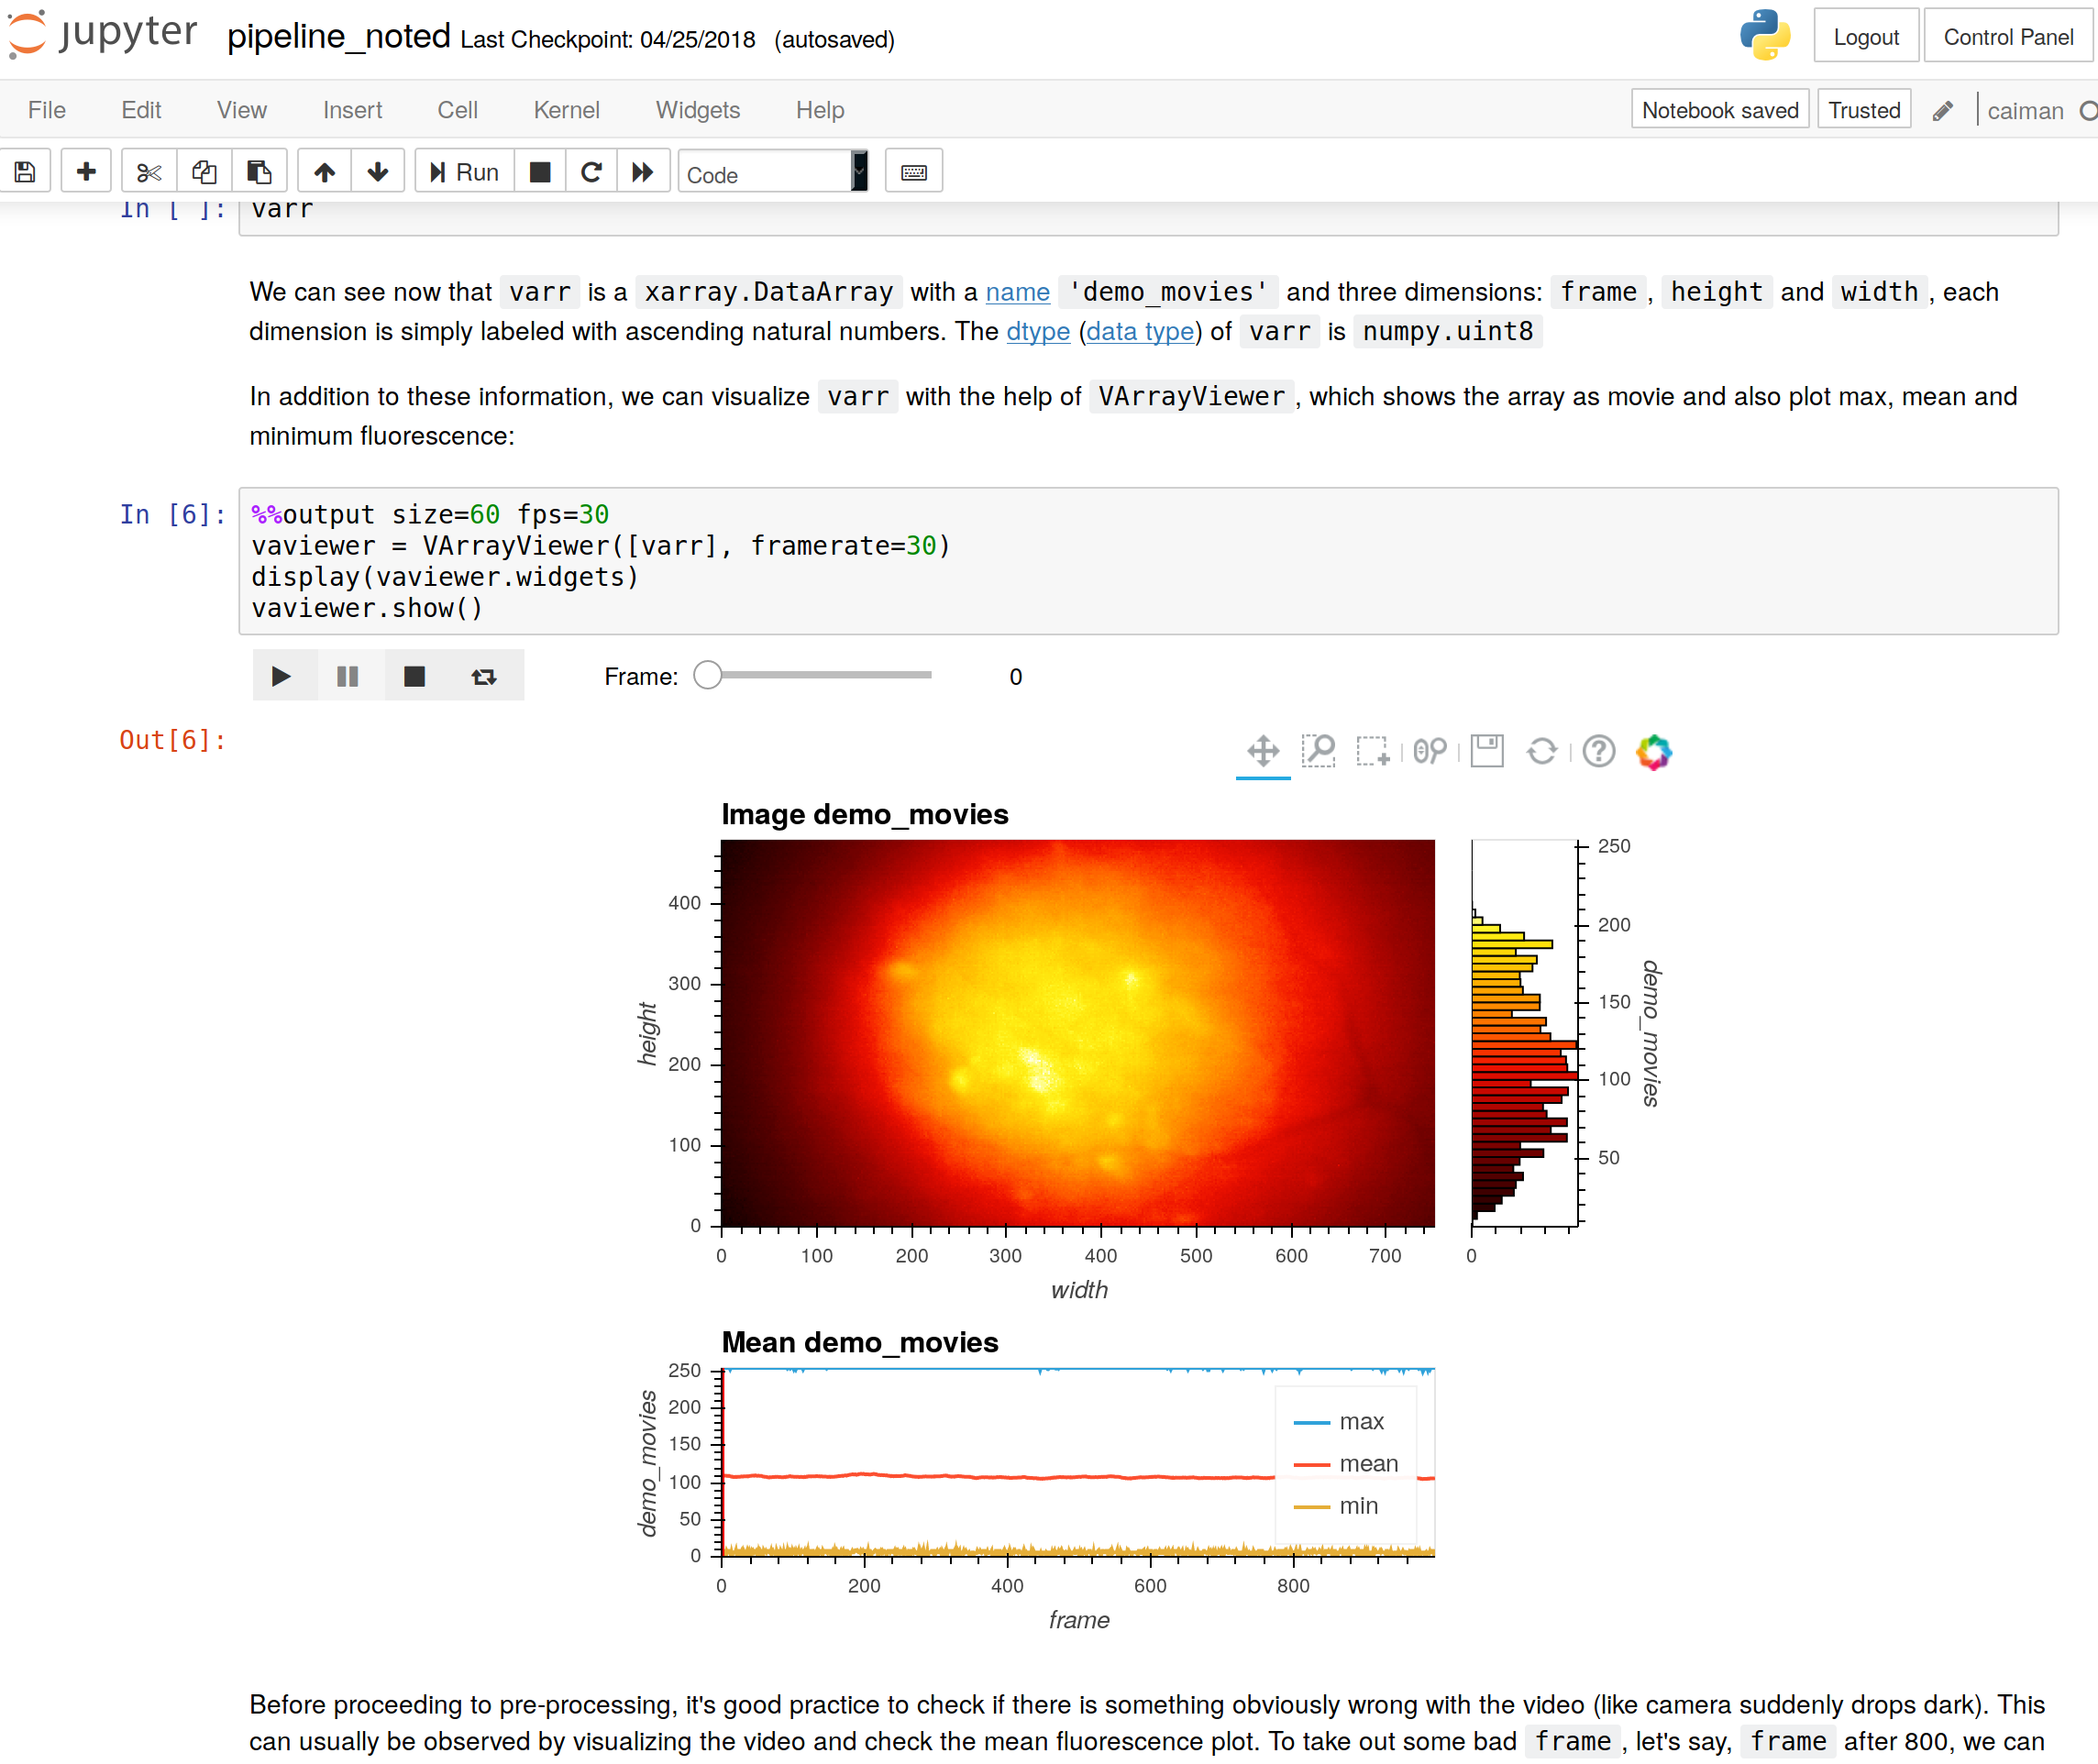
\includegraphics[scale = .13]{Figures/prelim_minian.png}
  \caption{\footnotesize integration of notes, codes and visualization of
  results in a single document.}
  \label{fig:prelim_minian}
\end{wrapfigure}

% \begin{figure}[!hbt]
%   \centering 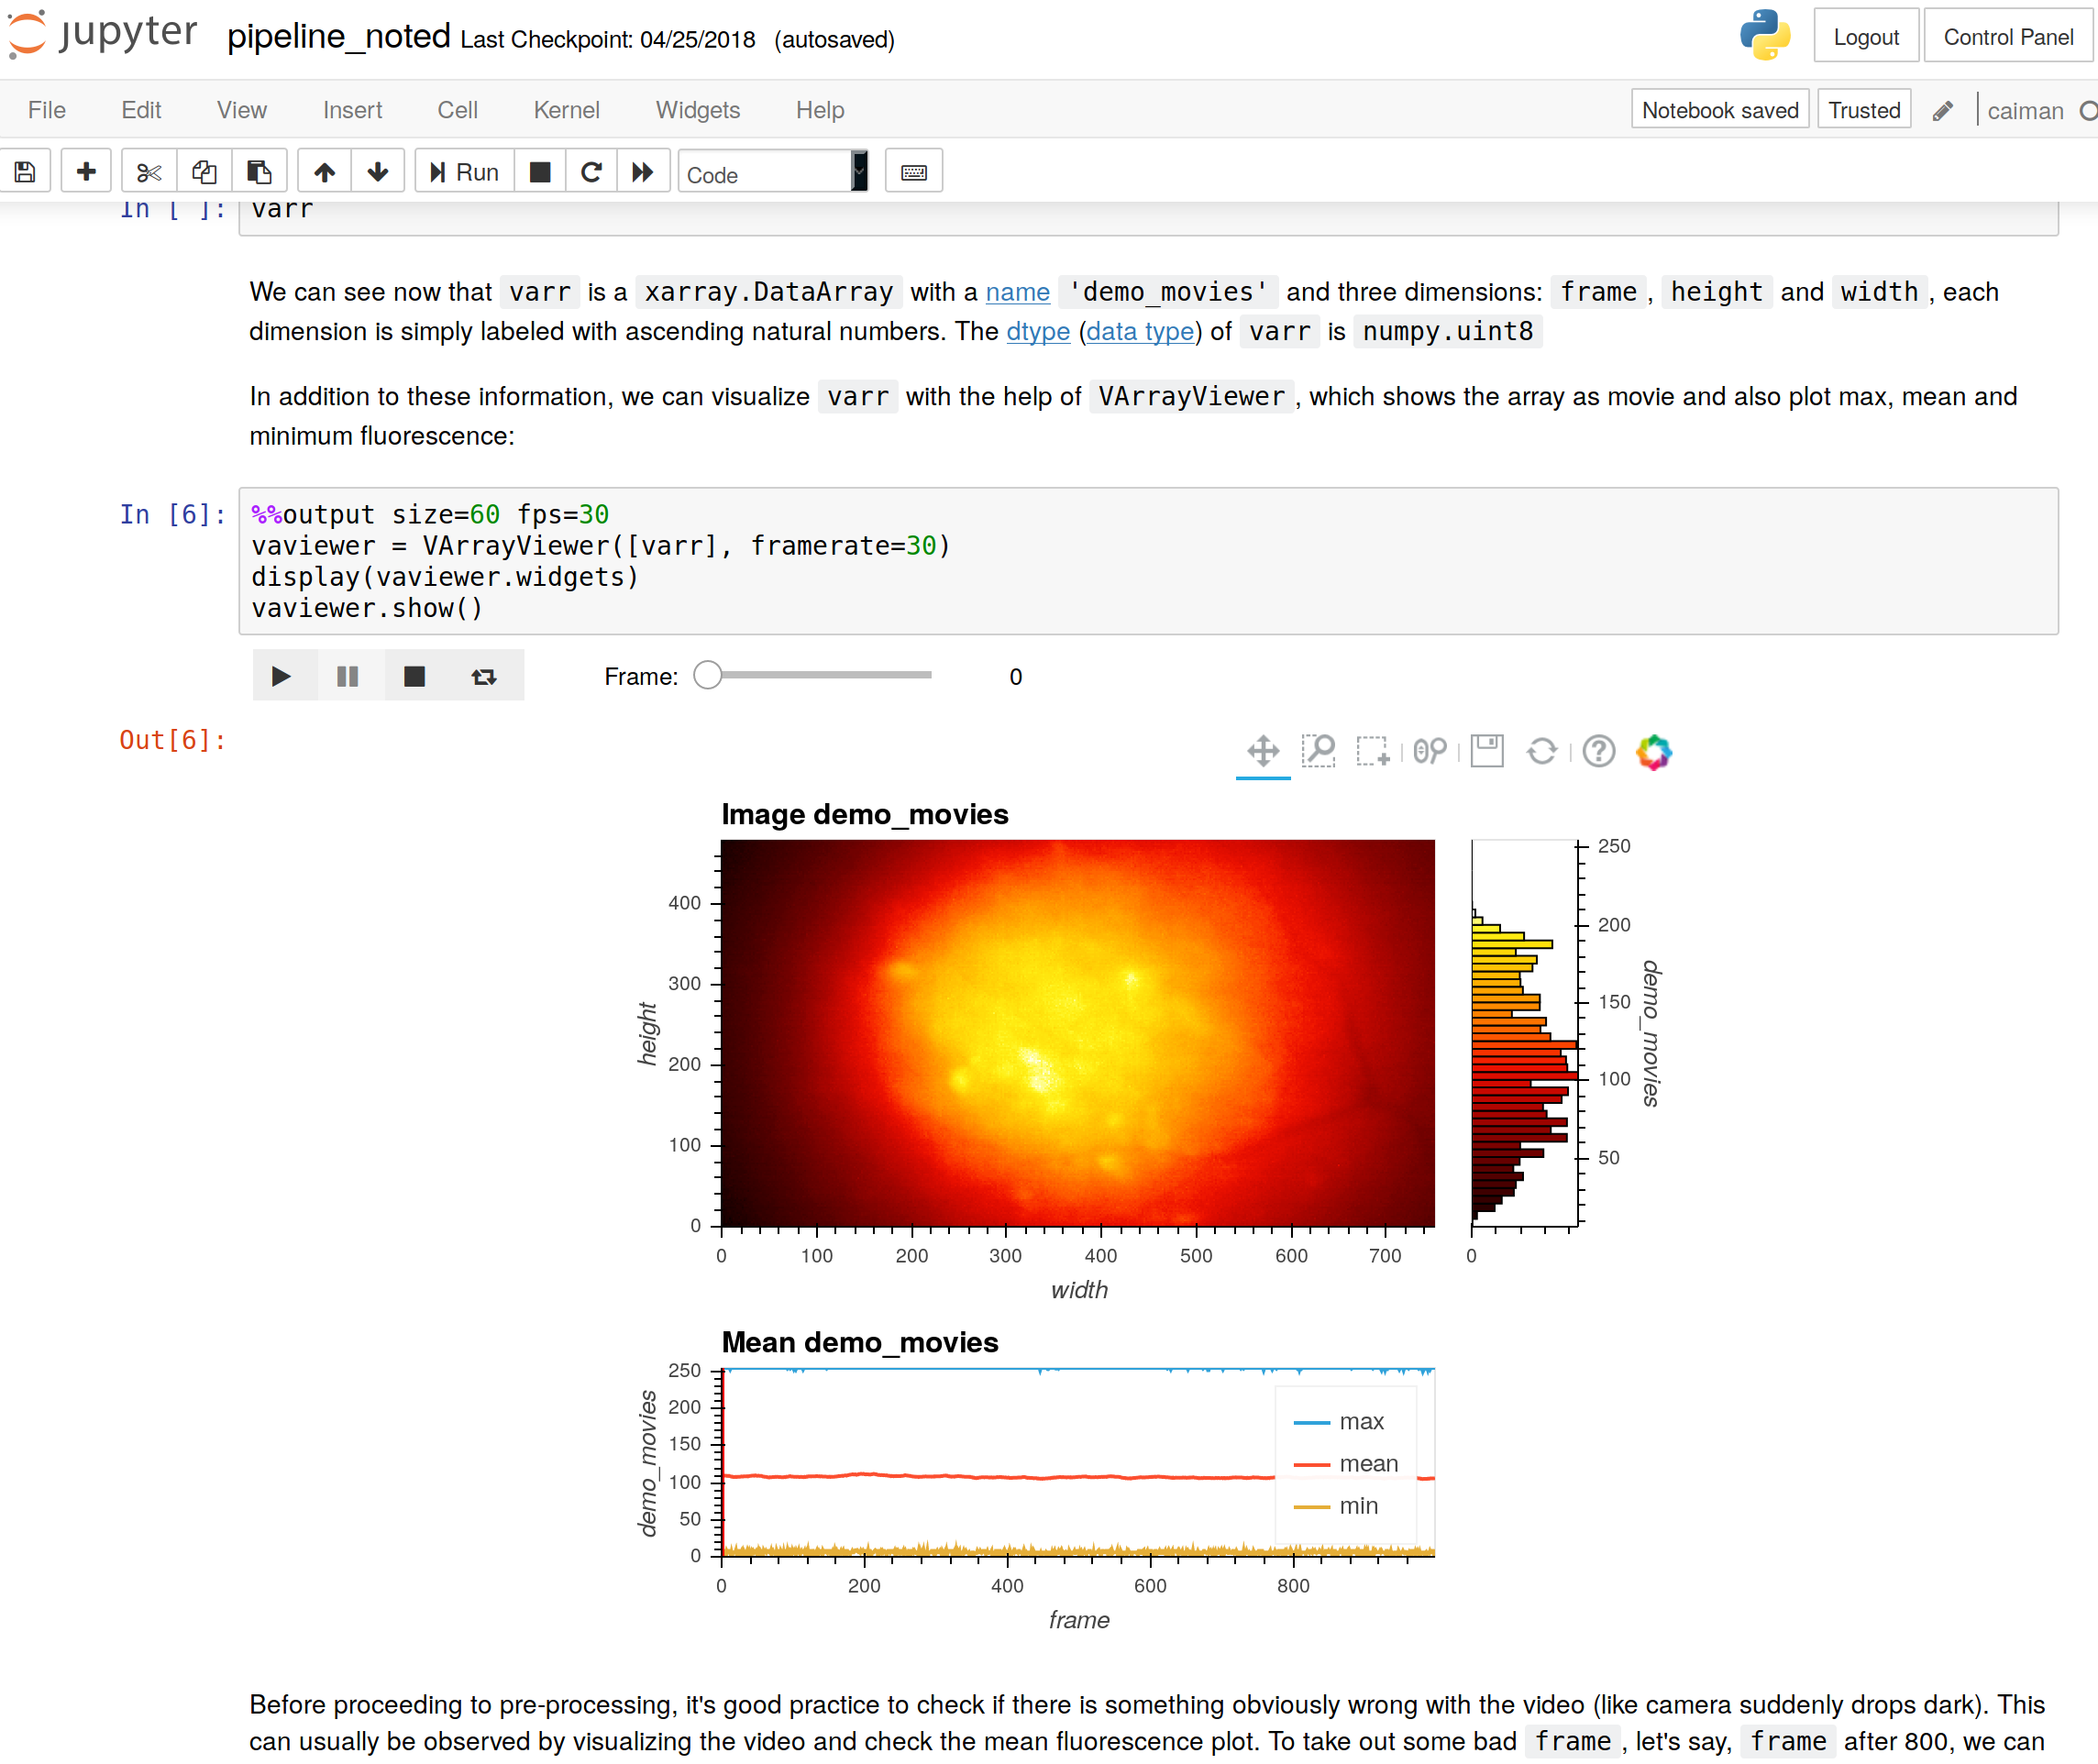
\includegraphics[scale = .135]{Figures/prelim_minian.png}
%   \caption{\footnotesize integration of notes, codes and visualization of
%     results in a single document.}
%   \label{fig:prelim_minian}
% \end{figure}

To address the difficulties raised during the analysis of calcium imaging data
with miniature microscopes, we have developed an open-source analysis pipeline
that allows the user to easily run through code, take notes and visualize the
results at the same time. Specifically, the pipeline incorporates pre--processing
steps that take raw videos as inputs, and corrects various artifacts that are
usually seen with miniature microscopes. For instance, the motion correction
step for miniature microscope is usually hindered by a ``dark ring'' around the
field--of--view caused by vignetting, ``bright spots'' caused by dust on the
lens or sensor, and a noise pattern that is stable across time. We apply various
interpolation and smoothing steps to specifically remove such artifacts before
motion correction, and the result of motion correction is improved. The results
from each step, including motion correction, can be visualized as
dynamically--generated animations (\textit{i.e.} without saving intermediate
videos to hard drives). Thus the user can easily visualize the effect of
pre--processing steps and decide whether each step is necessary for the specific
data. Regarding the result of the CNMF algorithm, there are two major concerns
about the quality of the extraction of calcium traces:
\begin{inparaenum}[a)]
\item the algorithm usually picks up ``units'' around the border of the
  field--of--view that are actually noise.
\item the balance between ``demixing'', where overlapping neurons are separated
  and treated as individual neurons, and ``merging'', where spatially scattered
  fluorescent signals coming from the same neuron are treated as single source,
  can be very sensitive to parameter tweaking, and it is often the case that
  signals coming from one neuron are falsely treated as separated neurons, or
  vice versa.
\end{inparaenum}
Thus, the pipeline also provides visualization tools to address these issues.
Specifically, the tools provide an overlaid contour plot of the spatial
footprints of all identified ``units'' within a session, thus the shape of each
``unit'' can be easily inspected. Moreover, the user can directly select
``units'' of interest from the overlaid contour plots, and the calcium traces of
selected ``units'' can be visualized in a manner that is similar to the plot of
spike trains of different neurons. Thus, the user can easily inspect whether
``units'' that are overlapping or close to each other have correlated calcium
traces that suggest a single source of signal. Furthermore, there is an option
to manually accept or reject ``units'' within the visualization tool, so that
the user can modify the results and take out false ``units'' without leaving the
visualization. All these features help the user to detect and correct the
potential pitfalls of the calcium signal extraction process. Finally, the whole
pipeline is provided as a jupyter notebook, which allows the user to easily take
and share text notes, edit and execute code, and dynamically visualize
results all in an integrated interface (\autoref{fig:prelim_minian}).

\end{document}
